% Created 2024-09-12 ju. 11:04
% Intended LaTeX compiler: pdflatex
\documentclass[aspectratio=169, usenames,svgnames,dvipsnames]{beamer}
\usepackage[utf8]{inputenc}
\usepackage[T1]{fontenc}
\usepackage{graphicx}
\usepackage{longtable}
\usepackage{wrapfig}
\usepackage{rotating}
\usepackage[normalem]{ulem}
\usepackage{amsmath}
\usepackage{amssymb}
\usepackage{capt-of}
\usepackage{hyperref}
\usepackage{color}
\usepackage{listings}
\usepackage[spanish]{babel}
\setbeamercolor{alerted text}{fg=Blue}
\setbeamerfont{alerted text}{series=\bfseries}
\setbeamercolor{block title}{bg=structure.fg!20!bg!50!bg}
\setbeamercolor{block body}{use=block title,bg=block title.bg}
\AtBeginSubsection[]{\begin{frame}[plain]\tableofcontents[currentsubsection,sectionstyle=show/shaded,subsectionstyle=show/shaded/hide]\end{frame}}
\AtBeginSection[]{\begin{frame}[plain]\tableofcontents[currentsection,hideallsubsections]\end{frame}}
\lstset{keywordstyle=\color{blue}, commentstyle=\color{gray!90}, basicstyle=\ttfamily\small, columns=fullflexible, breaklines=true,linewidth=\textwidth, backgroundcolor=\color{gray!23}, basewidth={0.5em,0.4em}, literate={á}{{\'a}}1 {ñ}{{\~n}}1 {é}{{\'e}}1 {ó}{{\'o}}1 {º}{{\textordmasculine}}1, showstringspaces=false}
\usepackage{mathpazo}
\hypersetup{colorlinks=true, linkcolor=Blue, urlcolor=Blue}
\usepackage{fancyvrb}
\DefineVerbatimEnvironment{verbatim}{Verbatim}{fontsize=\tiny, formatcom = {\color{black!70}}}
\usepackage{pgfplots}
\usetheme{Boadilla}
\usecolortheme{rose}
\usefonttheme{serif}
\author{Francisco Delgado López}
\date{}
\title{Desarrollo de una herramienta software para la simulación de sistemas fotovoltaicos con R}
\subtitle{Trabajo de Fin de Grado}
\institute[UPM]{Universidad Politécnica de Madrid}
\beamertemplatenavigationsymbolsempty
\setbeamertemplate{footline}[frame number]
\setbeamertemplate{itemize items}[triangle]
\setbeamertemplate{enumerate items}[circle]
\setbeamertemplate{section in toc}[circle]
\setbeamertemplate{subsection in toc}[circle]
\hypersetup{
 pdfauthor={Francisco Delgado López},
 pdftitle={Desarrollo de una herramienta software para la simulación de sistemas fotovoltaicos con R},
 pdfkeywords={},
 pdfsubject={},
 pdfcreator={Emacs 29.2 (Org mode 9.6.15)}, 
 pdflang={Spanish}}
\begin{document}

\maketitle

\section{Introducción}
\label{sec:org12c974c}
\subsection{Objetivos}
\label{sec:orgf14d9ee}
\begin{frame}[label={sec:orgf501f5a},fragile]{Objetivo principal}
 \begin{block}{Desarrollo de un paquete en \texttt{R}}
\begin{lstlisting}[numbers=left,language=r,label= ,caption= ,captionpos=b]
library(solaR2)
\end{lstlisting}
\end{block}
\end{frame}

\begin{frame}[label={sec:orgc431668},fragile]{Objetivos secundarios}
 \begin{block}{GNU Emacs}
\end{block}
\begin{block}{Paquetes de \texttt{R}}
\begin{itemize}
\item \texttt{solaR}
\item \texttt{zoo}
\item \texttt{data.table}
\item \texttt{microbenchmark}
\item \texttt{profvis}
\item \texttt{lattice}
\end{itemize}
\end{block}
\begin{block}{\LaTeX{}}
\end{block}
\begin{block}{Energía Solar Fotovoltaica}
\end{block}
\end{frame}

\section{Estado del arte}
\label{sec:orgc51f063}
\subsection{Sitación actual de la generación fotovoltaica}
\label{sec:orgbe3b03e}

\subsection{Soluciones actuales}
\label{sec:org27c6b1b}
\begin{frame}[label={sec:org1b38691}]{Soluciones actuales}
\begin{block}{\alert{PVsyst}}
\end{block}
\begin{block}{\alert{SISIFO}}
\end{block}
\begin{block}{\alert{PVGIS}}
\end{block}
\begin{block}{\alert{System Advisor Model}}
\end{block}
\end{frame}
\begin{frame}[label={sec:org4626c5c},fragile]{\texttt{solaR}}
 \begin{block}{Funcionamiento}
\begin{itemize}
\item Geometría solar
\item Datos meteorológicos
\item Radiación en el plano horizontal
\item Radiación en el plano del generador
\item Simulación de SFCR
\item Simulación de SFB
\item Optimización de distancias
\item Métodos de visualización
\end{itemize}
\end{block}
\end{frame}
\begin{frame}[label={sec:orgb35bd3f},fragile]{\texttt{solaR}}
 \begin{block}{Carencias}
\begin{itemize}
\item Modularidad
\item Eficiencia y rendimiento
\item Escalibilidad
\item Manipulación de datos
\end{itemize}
\end{block}
\end{frame}

\section{Marco teórico}
\label{sec:orgb2a662d}
\begin{frame}[label={sec:orgd5ef086}]{Procedimiento de cálculo}
\begin{center}
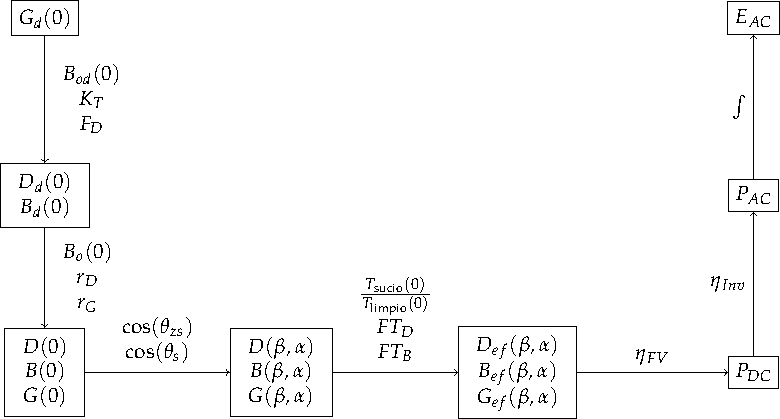
\includegraphics[scale=1]{../figuras/ProcedimientoCalculoRadiacionInclinada.pdf}
\end{center}
\end{frame}
\section{Desarrollo del código}
\label{sec:orgbd62322}
\subsection{Algorítmo de cálculo}
\label{sec:org44c12c6}
\begin{frame}[label={sec:orgddef758}]{Algorítmo de cálculo}
\begin{center}
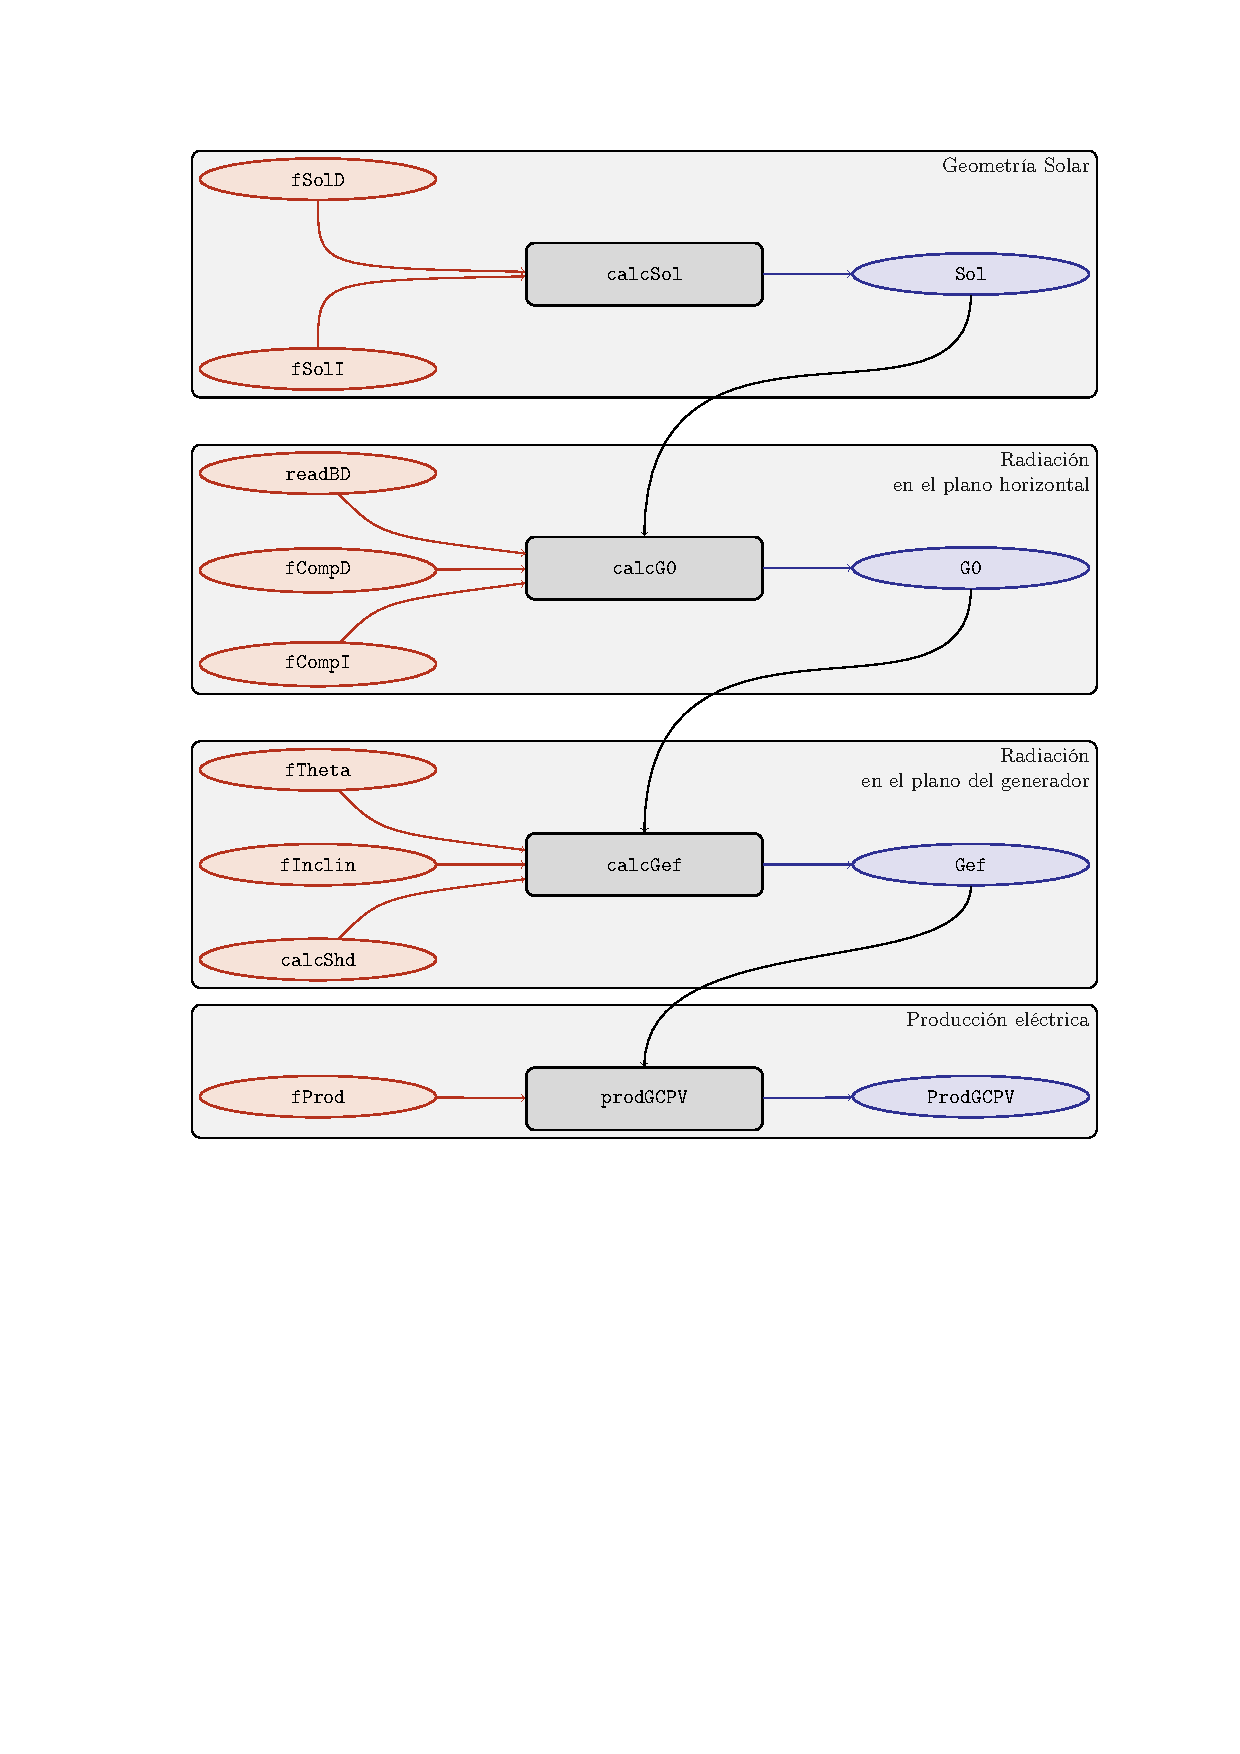
\includegraphics[height=0.9\textheight]{../figuras/procedure.pdf}
\end{center}
\end{frame}
\subsection{\texttt{calcSol}}
\label{sec:org2171daa}
\begin{center}
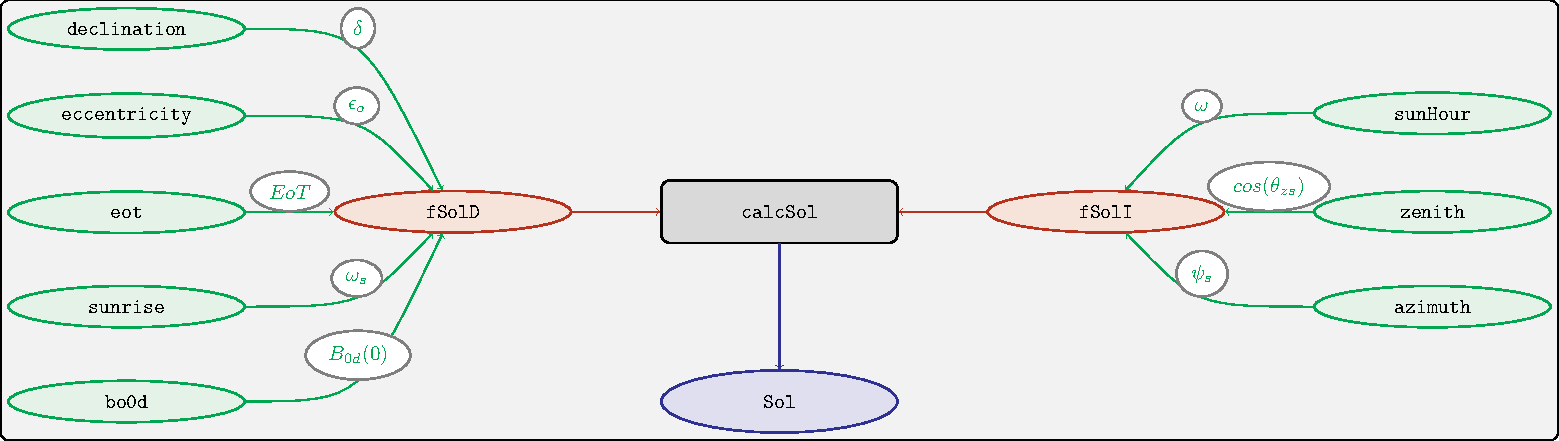
\includegraphics[scale=1]{../figuras/calcsol.pdf}
\end{center}
\begin{frame}[label={sec:org3e53a7d},fragile]{Ejemplo de uso}
 \begin{lstlisting}[numbers=left,language=r,label= ,caption= ,captionpos=b]
sol <- calcSol(lat = 37.2, BTd = '2024-01-17', sample = 'hour')
show(sol)
\end{lstlisting}
\end{frame}
\begin{frame}[label={sec:org3871619},fragile]{Ejemplo de uso}
 \begin{verbatim}
Object of class Sol 

Latitude:  37.2 degrees

Daily values:
     Dates                 decl               eo             EoT                 ws        
 Min.   :2024-01-17   Min.   :-0.3627   Min.   :1.034   Min.   :-0.04553   Min.   :-1.279  
 1st Qu.:2024-01-17   1st Qu.:-0.3627   1st Qu.:1.034   1st Qu.:-0.04553   1st Qu.:-1.279  
 Median :2024-01-17   Median :-0.3627   Median :1.034   Median :-0.04553   Median :-1.279  
 Mean   :2024-01-17   Mean   :-0.3627   Mean   :1.034   Mean   :-0.04553   Mean   :-1.279  
 3rd Qu.:2024-01-17   3rd Qu.:-0.3627   3rd Qu.:1.034   3rd Qu.:-0.04553   3rd Qu.:-1.279  
 Max.   :2024-01-17   Max.   :-0.3627   Max.   :1.034   Max.   :-0.04553   Max.   :-1.279  
      Bo0d     
 Min.   :4739  
 1st Qu.:4739  
 Median :4739  
 Mean   :4739  
 3rd Qu.:4739  
 Max.   :4739  

Intradaily values: 
     Dates                           w              night            cosThzS             AlS         
 Min.   :2024-01-17 00:00:00   Min.   :-2.92240   Mode :logical   Min.   :-0.9586   Min.   :-1.2819  
 1st Qu.:2024-01-17 05:45:00   1st Qu.:-1.41740   FALSE:10        1st Qu.:-0.7289   1st Qu.:-0.8172  
 Median :2024-01-17 11:30:00   Median : 0.08759   TRUE :14        Median :-0.2143   Median :-0.2160  
 Mean   :2024-01-17 11:30:00   Mean   : 0.08766                   Mean   :-0.2144   Mean   :-0.2724  
 3rd Qu.:2024-01-17 17:15:00   3rd Qu.: 1.59259                   3rd Qu.: 0.3003   3rd Qu.: 0.3051  
 Max.   :2024-01-17 23:00:00   Max.   : 3.09905                   Max.   : 0.5295   Max.   : 0.5580  
      AzS                Bo0       
 Min.   :-2.49463   Min.   :  0.0  
 1st Qu.:-1.18986   1st Qu.:  0.0  
 Median : 0.09526   Median :  0.0  
 Mean   : 0.08773   Mean   :197.0  
 3rd Qu.: 1.28896   3rd Qu.:424.5  
 Max.   : 3.00158   Max.   :748.4
\end{verbatim}
\end{frame}

\section{Ejemplo práctico de aplicación}
\label{sec:org4048c77}

\section{Conclusiones}
\label{sec:org2ab48e8}
\end{document}
